%\documentclass[11pt]{report}



%\begin{document}

\chapter{Technical overview}
%\addcontentsline{toc}{chapter}{Introduction}

Throughout this thesis, Alice plays the role of the sender and Bob plays the role of the receiver.


\section{Mathematical preliminaries}

We denote by $\gcd (a,b), a,b\in\mathbb{Z}$ the greatest common divisor between integers $a$ and $b$. $\mathbb{Z}_q$ denotes the set of integers $a \mod q$. $\mathbb{Z}^*_q$ is the set of integers $a\in\mathbb{Z}_q$ that are coprime with $q$, i.e. $\gcd (a,q) = 1$. For $q$ prime, $\mathbb{Z}^*_q$ forms a multiplicative group of order $q-1$ and $\mathbb{Z}_q$ a finite field of order $q$. A generator $g$ of some multiplicative group $\mathbb{G}$ is an element in $\mathbb{G}$ such that $\forall\,a\in\mathbb{G}, \exists r\, :\, g^r = a$. The discrete logarithm base $g$ of some element $a\in\mathbb{G}$, denoted by $\log_g a$, is the power $r$ of $g$ such that $g^r = a$. 

We use $|I|$ to denote the size of a set $I$. We use the notation $s\leftarrow_{\$}I$ to describe a situation where an element $s$ is drawn uniformly at random from the set $I$. For some set $J$, $\bm{v}_J$ denotes the subvector of $\bm{v}$ restricted to the indexes of set $J$. Let $\mathbb{Z}_q$ denote the finite field with order $q$. Then, for $m\in \mathbb{Z}_q$, $[m]$ is the ordered set $\{1, 2, \ldots, m\}$. Also, for $m, n\in \mathbb{Z}_q$ such that $m<n$, $[m, n] = \{m, m+1, \dots, n-1, n\}$. Also, we use the big-$\mathcal{O}$ notation to denote the fastest-growing term of the number of operations with respect to some security parameter $n$.



%********************************** %First Section  **************************************
\section{Secure multiparty computation}

Let us consider a scenario with $n$ parties, $P_i$, each with input $x_i$, $i\in \{ 1, ..., n\}$. Simply put, secure multiparty computation (SMC) allows these $n$ parties to jointly compute some function, $f( x_1, ..., x_n ) = (y_1, ..., y_n)$, without revealing about their inputs more than what can be infered by the input-output behaviour. This functionality is designed to be equivalent to a scenario where every party, $P_i$, sends his inputs, $x_i$, to some independent and trusted third party, $P_{\mathsf{TTP}}$, who computes $f( x_1, ..., x_n )$ and sends back to each party their corresponding output, $y_i$.

We stress that in SMC it may not be possible to fully hide the inputs from the other parties, even with a perfectly maliciously secure protocol. This comes from the security guarantees covered by the ideal scenario. Indeed, there could be the case where a perfectly legitimate SMC protocol (e.g. using a trusted third party) leaks the inputs of the parties. This happens when one of the parties can use the output and his inputs to invert the function $f()$. As an example, imagine that two people want to compute the average of the weight of each other. It is straightforward to see that both parties can use their weight and the average value to compute the other party's weight. This always happens whenever $f()$ is bijective with the adversaries' inputs fixed. In this scenario, SMC does not improve the privacy of the computation. 
%Estrutura da introdução:
%
%- Cometar que não sabemos mais do que o output da computação. Dar o exemplo da média de pesos. 2 pessoas sabemos o resultado. 3 já não. Ainda assim, pode revelar alguma coisa a mais. Note that, pratically, we can put together other PET such as Differential Privacy in oder to do this.

The following are some properties of SMC which we informally describe:

\begin{enumerate}
\item Correctness: if all the parties do not deviate from the protocol, the protocol evaluates the correct output according to $f()$ and the parties' inputs $x_1, \ldots, x_n$;

\item Passive security: even if the adversaries do not deviate from the protocol, they do not learn the inputs of the honest parties. Throughout this thesis, we refer to adversaries who do not deviate from the protocol as semi-honest parties. In the literature, these are also called honest-but-curious adversaries.

\item Active security: even if the adversaries deviate arbitrarily from the protocol, they do not learn the inputs of the honest parties. In active security there are two types of protocols that react differently with respect to the adversarial behaviour. They can be robust against the advarsaries, meaning the honest parties will still receive the correct answer. Or honest parties abort the protocol when there exists some malicious activity.
\end{enumerate}

Regarding the corruption strategy of the adversaries, they can be of two types: static or adaptive. Static security guarantees that the protocol is secure against an adversary who only corrupts parties before the execution of the protocol. Adaptive security is an harder property to attain as it assumes that the adversary can choose throughout the protocol the party to be corrupted.

Also, it is interesting to note that there is a fundamental difference between the adversarial structure of encryption methods and SMC methods. In encryption methods, the adversary is not part of the protocol. It is considered as an external party (usually called Eve) that interfeers with the communication between the protocol parties. In the case of SMC methods, the adversaries are a subset of the protocol parties.

%Talk about two approaches: boolean and arithmetic. Discuss the advantages and disadvantages of each.

\subsection{Boolean approach}

Boolean approach is based on the Yao protocol. In order to do it we need OT. We start by presenting OT and then we describe the Yao protocol.


\subsubsection{Oblivious transfer}

The study of oblivious transfer (OT) has been very active since its first proposal in 1981 by Rabin \cite{Rabin81}. The importance of OT comes from its wide number of applications. More specifically, one can prove that OT is equivalent to the secure two-party computation of general functions \cite{Y86, K88}, i.e. one can implement a secure two-party computation using OT as its building block. Additionally, this primitive can also be used for secure multi-party computation (SMC) \cite{KOS16}, private information retrieval \cite{Che04}, private set intersection \cite{MEP17}, and privacy-preserving location-based services \cite{BHM+19}.


\begin{figure}[h!]
\centering
\begin{tcolorbox}[enhanced, 
                        frame hidden,
                        ]
                        
    \centerline{$\mathcal{F}_{\textbf{OT}}$ \textbf{functionality}}
            
    \
    
    \begin{itemize}
    		\item \textbf{Input phase:} Alice sends $(m_0, m_1)\in\{0,1\}^l$ (two messages) to $\mathcal{F}_{\textbf{OT}}$ and Bob sends $b\in\{0,1\}$ (bit choice) to $\mathcal{F}_{\textbf{OT}}$.
    		\item \textbf{Output phase:} Alice receives nothing $\bot$ from the functionality and Bob receives $m_b$.
    \end{itemize}
    
\end{tcolorbox} 
    \caption{OT functionality.}
    \label{fig:OT_functionality}
\end{figure}

The OT functionality specification is presented in Figure~\ref{fig:OT_functionality}. Consequently, we have that OT must satisfy the following security requirements:

\begin{itemize}
	\item Concealing: Alices knows nothing about Bob's bit choice $b$.
	\item Obliviousness: Bob knows nothing about the message $m_{b\oplus 1}$.
\end{itemize}

The above OT functionality (Figure~\ref{fig:OT_functionality}) is commonly called $1$-out-of-$2$ OT. Thus, it can be generalized to the case of $k$-out-of-$N$ OT, where Alice owns $N$ messages, and Bob can choose $k$ of them. For $k=1$, this is commonly called private database query (PDQ). 

\subsubsection{Yao protocol}\label{yaoProtocol}

A solution to SMC was given for the first time by Yao \cite{Yao82} and its main idea resides on the fact that every function has a boolean circuit representation. From this, Yao developed the concept of garbled circuits which is one of the key elements for secure computation. The Yao's garbled circuit protocol is constrained to only two parties but its generalization was achieved by GMW \cite{Goldreich87}, BGW \cite{BGW88, CCD88} and BMR \cite{BMR90}. Also, some implementation optimizations on Yao protocol were later developed in order to improve its performance: point-and-permute \cite{BMR90}, row reduction \cite{NPS99, Pinkas2009}, FreeXOR \cite{Kolesnikov2005} and half gates \cite{Zahur2015}. 

As we said before, the main idea of Yao protocol is to represent the desired function $f()$ as a boolean circuit $C$, i.e. by a sequence of logical gates interconnected with wires. After the generation of the circuit $C$, each party will have two very different roles. Generally speaking, one of the parties Alice (usually called garbler) randomly generates keys to each input bit, encrypts each circuit's gate and sends both elements to Bob (called evaluator). This procedure masks Alice's inputs from Bob. Then, through the OT functionality, Bob receives the keys corresponding to his input bits. So, OT allows to mask Bob's inputs from Alice. Finally, since the evaluator has all the input keys, he can decrypt every gate, i.e. evaluate the circuit. Let us see in more detail how the protocol works using a four input boolean circuit description of the Millionaires' problem. This problem can be described by the following expression:

\begin{equation}
f(a, b) = 
     \begin{cases} 
      1 & \mathrm{if} \hspace{0.2cm} a>b, \\
      0 & \mathrm{otherwise},
   \end{cases}
\label{eq:MPeq}
\end{equation}   
for $a, b \in \{0,1\}^2$. In summary, it allows two parties to discover who input the largest value without revealing their inputs.

The protocol goes as follows:
\begin{enumerate}
    \item \textit{Circuit generation:} The garbler Alice generates a boolean circuit of function (\ref{eq:MPeq}):
    
    \begin{figure}[h]
        \centering
        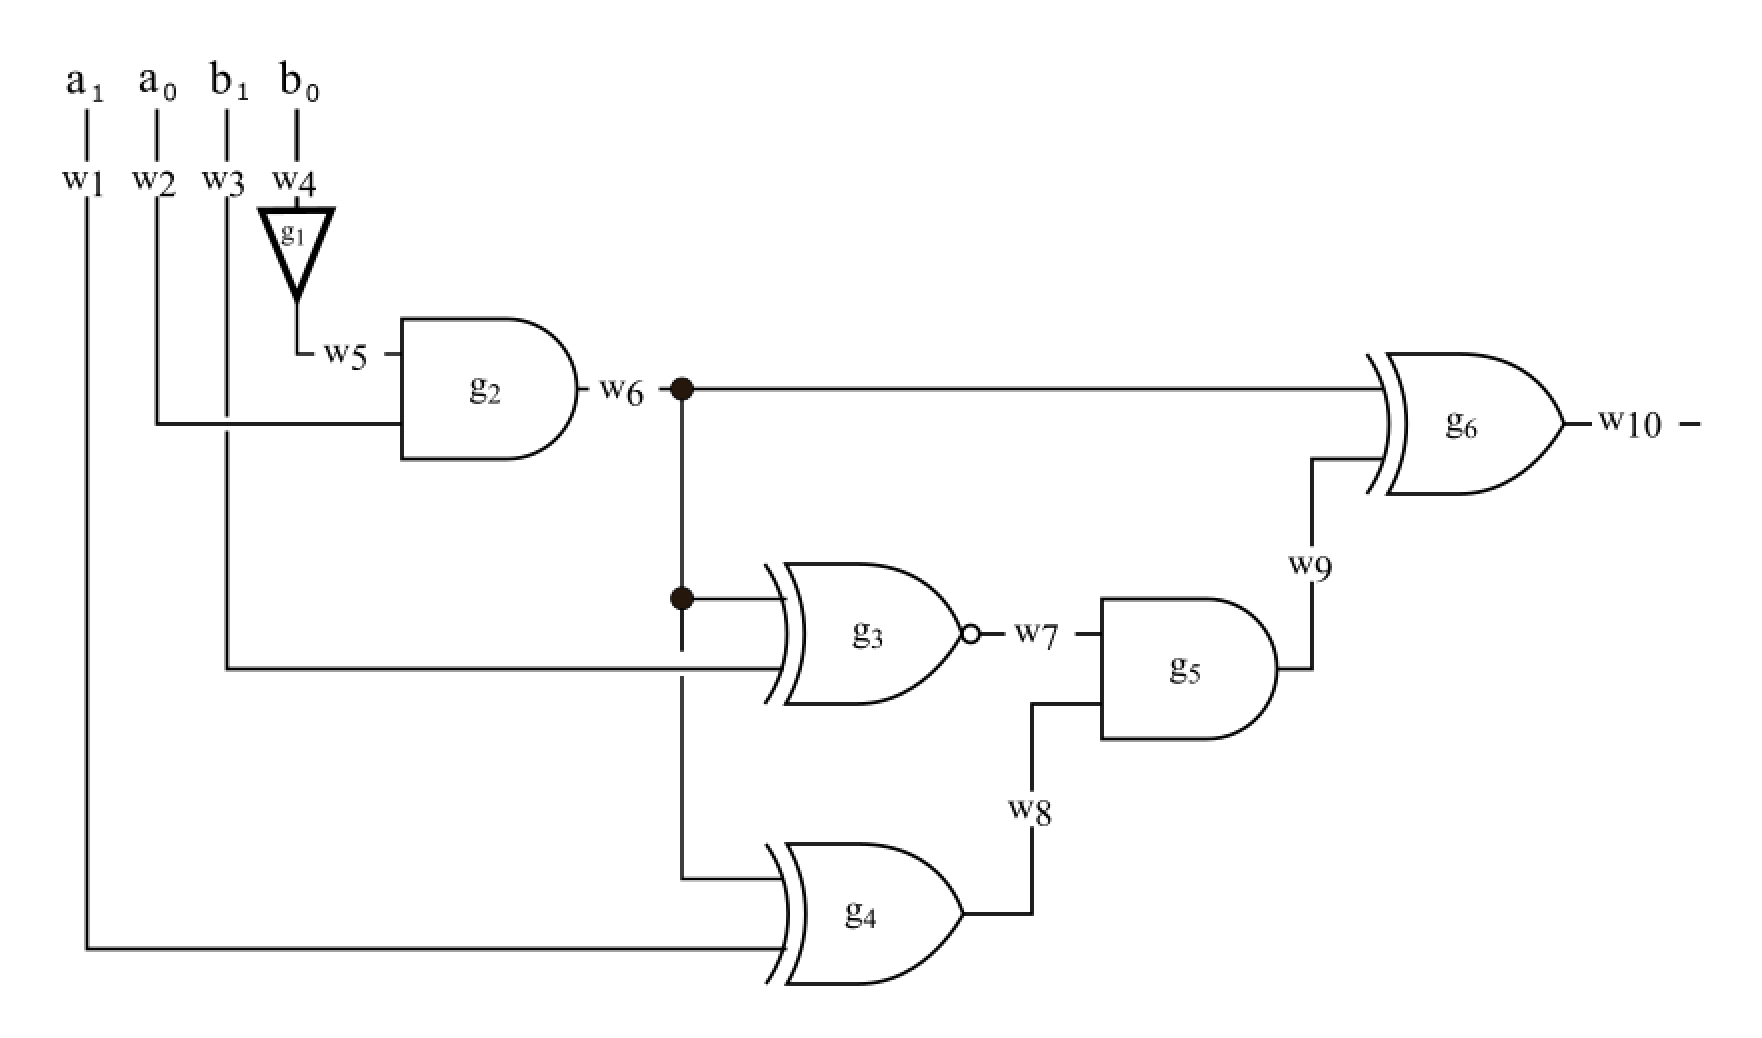
\includegraphics[scale=0.4]{Chapter_TechnicalOverview/booleanCircuit.png}

        \caption{Boolean circuit of the Millionaires' Problem. Optimized circuit according to the construction in \cite{Kolesnikov2009}.}
        \label{fig:boolean}
    \end{figure}
    
    In this case, the circuit contains one NOT gate ($g_1$), two AND gates ($g_2$, and $g_5$), two XOR gate ($g_4$ and $g_6$), one XNOR gate ($g_3$) and four input wires ($w_1$ and $w_2$ belongs to Alice and $w_3$ and $w_4$ to Bob).
    
    \item \textit{Wire encryption:} Alice uses a random number generator to generate two keys $k^0_i$ and $k^1_i$ for each wire $w_i$, $i\in\{1, ..., 10\}$. These keys correspond to the possible values ($0$ or $1$) on the wire. Note that this is done to prevent Bob from knowing the true value of the wires during the evaluation process.
    
    \item \textit{Gate encryption:} For every gate $g_l$ in the circuit with corresponding input wires $w_i$ and $w_j$ and output wire $w_s$, Alice creates the following table:
    
    \

    \begin{center}
        \begin{tabular}{ |c| } 
        \hline
        $\mathsf{Enc}_{k_i^0}\left(\mathsf{Enc}_{k_j^0}\left(k_s^{g_l(0,0)}\right)\right)$ \\ 
        \hline
        $\mathsf{Enc}_{k_i^0}\left(\mathsf{Enc}_{k_j^1}\left(k_s^{g_l(0,1)}\right)\right)$ \\ 
        \hline
        $\mathsf{Enc}_{k_i^1}\left(\mathsf{Enc}_{k_j^0}\left(k_s^{g_l(1,0)}\right)\right)$ \\ 
        \hline
        $\mathsf{Enc}_{k_i^1}\left(\mathsf{Enc}_{k_j^1}\left(k_s^{g_l(1,1)}\right)\right)$ \\
        \hline
        \end{tabular}
    \end{center}
    
    where $g_l(t,r)$ is the output of gate $g_l$ for inputs $t, r\in \{0, 1\}$. So, we could think of each row as a locked box that requires two keys to be opened. If the two correct keys are used, it outputs the key corresponding to the desired output value given by $g_l$. After encrypting each gate, Alice permutes the rows of the corresponding table, otherwise, it would be easy to know the real value of the input keys. Then, she sends to Bob the garbled tables along with Alice's input keys.
    
    \
    
    As an example, we can easily see that if we use input keys $k_i^0$ and $k_j^1$ (corresponding to real values $0$ and $1$), we would only be able to decipher the second row of the table, $\mathsf{Enc}_{k_i^0}(\mathsf{Enc}_{k_j^1}(k_s^{g_l(0,1)}))$, and get $k_s^{g_l(0,1)}$.
    
    
    \item \textit{Oblivious Transfer:} At this stage of the protocol, the evaluator Bob knows the garbled circuit and Alice's input keys but he does not know the keys corresponding to his real inputs. However, since Bob wants to keep his input value private he cannot directly ask for those keys. At this point, the OT functionality enables the evaluator to receive his input keys without compromising neither the evaluator's nor garbler's security. In fact, for every input wire, both parties perform an OT where Alice plays the role of sender and Bob plays the role of receiver. 
    
    \
    
    Let us assume Alice's input keys to be $k_1^0$ and $k_2^1$ (corresponding to the real value  $01$) and Bob's input bits to be $11$. This means that Bob must use the respective input keys ($k_3^1$ and $k_4^1$) in order to correctly evaluate the circuit. So, they will execute two OT protocols where:
    
    \begin{itemize}
        \item Alice inputs: $(k_3^0, k_3^1)$ and $(k_4^0, k_4^1)$;
        \item Bob inputs: $b_1 = 1$ and $b_2 = 1$.
    \end{itemize}
    
    \item \textit{Evaluation:} Once the evaluator has all the necessary elements, he can proceed with the circuit evaluation. In this step, he simply has to decipher the correct rows of the garbled tables sent by Alice with the corresponding keys. Since the rows of the tables are shuffled, the evaluator does not know which row is the correct one. This small issue can be solved by simple techniques (Point-and-Permute or encryption with a certain number of $0$ padded) which, for the sake of brevity, we will not explore here. At the end of the evaluation, the evaluator receives the key that corresponds to the result. Finally, the evaluator sends the resulting key to the garbler and the garbler tells him the final bit.
    
    \
    
    According to our Millionaires' problem, the evaluation yields the following results for $a = 01$ and $b = 11$: $g_1(k_4^1) = k_5^0$, $g_2(k_5^0, k_2^1) = k_6^0$, $g_3(k_6^0, k_3^1) = k_7^0$, $g_4(k_6^0, k_1^0) = k_8^1$, $g_5(k_7^0, k_8^1) = k_9^0$, $g_6(k_6^0, k_9^0) = k_{10}^0$. Actually, the desired result is $0$.
    
\end{enumerate}


The Yao protocol has its security based on two main building blocks: garbled circuits and oblivious transfer. Although garbled circuits can be generated with symmetric encryption (i.e. using double AES encryption), OT protocols cannot be classically achieved with symmetric cryptography alone \citep{IR89}. Thus, it is crucial to find efficient protocols for a quantum-resistant OT.

%Lindell and Pinkas presented a simulation-based proof that is based on the fact that 
%LP09


%Description
%
%Optimizations
%
%Security
%
%Generalizations of Yao: GMW, BMR

\subsection{Arithmetic approach}



\subsubsection{Oblivious linear evaluation}

The study of oblivious transfer (OT) has been very active since its first proposal in 1981 by Rabin \cite{Rabin81}. The importance of OT comes from its wide number of applications. More specifically, one can prove that OT is equivalent to the secure two-party computation of general functions \cite{Y86, K88}, i.e. one can implement a secure two-party computation using OT as its building block. Additionally, this primitive can also be used for secure multi-party computation (SMC) \cite{KOS16}, private information retrieval \cite{Che04}, private set intersection \cite{MEP17}, and privacy-preserving location-based services \cite{BHM+19}.


\begin{figure}[h!]
\centering
\begin{tcolorbox}[enhanced, 
                        frame hidden,
                        ]
                        
    \centerline{$\mathcal{F}_{\textbf{OLE}}$ \textbf{functionality}}
            
    \
    
    \begin{itemize}
    		\item \textbf{Input phase:} Alice sends $(a,b)\in\mathbb{Z}_d^2$ (two field elements) to $\mathcal{F}_{\textbf{OLE}}$ and Bob sends $x\in\mathbb{Z}_d$ to $\mathcal{F}_{\textbf{OLE}}$.
    		\item \textbf{Output phase:} Alice receives nothing $\bot$ from the functionality and Bob receives $f(x):= ax + b$.
    \end{itemize}
    
\end{tcolorbox} 
    \caption{OLE functionality.}
    \label{fig:OLE_functionality}
\end{figure}

The OLE functionality specification is presented in Figure~\ref{fig:OLE_functionality}. Similarly, we have that OLE must satisfy the following security requirements:

\begin{itemize}
	\item Concealing: Alices knows nothing about Bob's field element $x$.
	\item Obliviousness: Bob knows nothing about the function $f()$ other than its evaluation at $x$, i.e. $f(x)$.
\end{itemize}

We can also generalize to the OLE functionality to a vectorized version. The vector OLE functionality is presented in Figure~\ref{fig:VOLE_functionality}. Note that Bob only inputs one field element $x$ and Alice inputs two vectors. 


\begin{figure}[h!]
\centering
\begin{tcolorbox}[enhanced, 
                        frame hidden,
                        ]
                        
    \centerline{$\mathcal{F}_{\textbf{VOLE}}$ \textbf{functionality}}
            
    \
    
    \begin{itemize}
    		\item \textbf{Input phase:} Alice sends $(\bm{a},\bm{b})\in\mathbb{Z}_d^{2n}$ (two vectors of field elements) to $\mathcal{F}_{\textbf{VOLE}}$ and Bob sends only $x\in\mathbb{Z}_d$ to $\mathcal{F}_{\textbf{VOLE}}$.
    		\item \textbf{Output phase:} Alice receives nothing $\bot$ from the functionality and Bob receives $\bm{f}(x):= \bm{a}x + \bm{b}$.
    \end{itemize}
    
\end{tcolorbox} 
    \caption{VOLE functionality.}
    \label{fig:VOLE_functionality}
\end{figure}

\subsubsection{SPDZ}





%********************************** %Second Section  **************************************
\section{Quantum Information}

$\mathcal{B}(\mathcal{H})$ is the set of positive semi-definite operators with unitary trace acting on an Hilbert space $\mathcal{H}$. {\cv It is used in chapter 3.2.5 Noisy-quantum-storage model}

\subsection{Quantum states representation}

\subsection{Entropy}

\subsection{Two-universal functions}

\subsection{Mutually Unbiased Basis}




%********************************** %Third Section  **************************************
\section{Universal Composability}


%********************************** %Fourth Section  **************************************
\section{Functionality definitions}


%\bibliography{bibforthesis}
%\bibliographystyle{unsrt}
%\end{document}
